\documentclass[a4paper]{article}

%% Language and font encodings
\usepackage[T1]{fontenc}
\usepackage[utf8x]{inputenc}
\usepackage[english]{babel}

\usepackage[colorlinks=true, allcolors=blue]{hyperref}

\urlstyle{tt}
\newcommand{\email}[1]{\href{mailto:#1}{\tt{\nolinkurl{#1}}}}
\newcommand{\orcid}[1]{ORCID: \href{https://orcid.org/#1}{\tt{\nolinkurl{#1}}}}

\newcommand{\figleg}[1]{\centering\itshape{#1}\/}
\newcommand{\figref}[1]{ (see figure~\ref{#1})}
%\newcommand{\eqref}[1]{ (see equation~\ref{#1})}

\usepackage[sfdefault,lf]{carlito}
%% The 'lf' option for lining figuressy
%% The 'sfdefault' option to make the base font sans serif
\usepackage[parfill]{parskip}
\renewcommand*\oldstylenums[1]{\carlitoOsF#1}%
\usepackage{fancyhdr}
\usepackage{natbib}
\usepackage{authblk}
\setlength{\headheight}{41pt}

%% Sets page size and margins
\usepackage[a4paper,top=3cm,bottom=2cm,left=3cm,right=3cm,marginparwidth=1.75cm]{geometry}

%% Useful packages
\usepackage{amsmath}
\usepackage{graphicx}
\usepackage{booktabs}
\usepackage{caption}
\usepackage{subcaption}

\usepackage[colorinlistoftodos]{todonotes}

\fancyhead[L]{Posted: \today}
\fancyhead[R]{

\includegraphics[width=4cm]{img/engrXiv_banner.png}
}
\pagestyle{plain}
\title{Adaptive Removal of the Transcranial Alternating Current Stimulation Artifact from the Electroencephalogram}
\author[1,*]{Robert Guggenberger}
\author[1]{N.N.}
\affil[1]{Department for Translational Neurosurgery, University Hospital Tübingen}

\affil[*]{Corresponding author: \email{robert.guggenberger@posteo.eu}}
\date{\today}

\usepackage{varioref}
\usepackage{hyperref}
\usepackage{cleveref}
\hypersetup{hidelinks = true}

\usepackage[nonumberlist,acronym]{glossaries}
% abbreviations:
\newacronym{eeg}{EEG}{electroencephalogram}
\newacronym{tacs}{tACS}{transcranial alternating current stimulation}
\newacronym{tms}{TMS}{transcranial magnetic stimulation}
\newacronym{tpca}{tPCA}{temporal principal component analysis}
\newacronym{sma}{SMA}{superposition of moving averages}
\makeglossaries{}

% --------------------------------------------------------------------------
\begin{document}
\maketitle
\thispagestyle{fancy}

\begin{abstract}
Your abstract.
\end{abstract}

\section{Introduction}

The combination of \gls{tacs} and \gls{eeg} has been explored in several recent studies. While the analysis of \gls{eeg} before or after stimulation posits limited technical challenges, the \gls{eeg} recording during stimulation is heavily affected by the stimulation artifact.

\subsection{Matched Phase and Frequency}
Computational simulations suggest that the power of endogenous oscillations would increase most if the frequency of~\gls{tacs} matches the targets eigenfrequency~\citep{Kutchko_2013,Zaehle_2010}.
This has been supported by evidence from animal studies~\citep{Schmidt_2014}, and human studies combining \gls{tacs} with \gls{tms} \citep{Guerra_2016}, or contrasting pre and post resting state power analysis \citep{Zaehle_2010}.
It has also been suggested that the phase of neuronal populations would be locked to the phase of the \gls{tacs} signal \citep{Reato_2013}. This has been supported by evidence from studies combining \gls{tacs} with motor output \citep{Brittain_2013}, \gls{tms}~\citep{Raco_2016,Nakazono_2016} or sensory perception~\citep{Gundlach_2016}.

This suggests that the effect of \gls{tacs} can result in neurophysiological effects which are phase-and frequency-matched to the stimulation artifact. Such frequency and phase matching between \gls{tacs} and \gls{eeg} recordings can render the removal of the artifact difficult or impossible, as the signal might no longer be separatable from the artifact.

\subsection{Non-Stationary Amplitude Modulation}

An approach to tackle this issue is to assess the time-course of the~\gls{eeg} signal. Consider the assumption that the artifact is stationary and superpositioned on the physiological signal. Then, modulations in the amplitude of the recorded~\gls{eeg}-signal must be caused by changes in the underlying physiology.
This would be the case, even if frequency and phase are matched to the stimulation signal. Approaches assuming such stationarity of the stimulation artifact have been used e.g.\ by~\cite{Pogosyan_2009}.

Yet, detailed analysis of the stimulation artifact provides evidence that the artifact amplitude is actually not stationary. Instead, the amplitude is modulated by heart-beat and respiration~\citep{Noury_2016}. It has been argued that unregularized spatial filters might be able to remove this amplitude modulation~\citep{Neuling_2017}. But if only few channels are recorded, the method can fail, as the estimation of the spatial covariance is insufficient, or impossible in the single-channel-case.
Consider furthermore that event-related responses like modulation of skin impedance can also affect the scalp conductance at stimulation electrodes. This would introduce event-related amplitude modulation of the stimulation artifact. In that regard, disentangling true signal from the stimulation artifact stays technically challenging.

\subsection{Artifact Distortion}

Ideally, the stimulation artifict of~\gls{tacs} resembles a sinusoid. Yet, practical experience suggests that the signal is usually distorted to various degrees.
Figure~\ref{fig:nonsinus} shows examples of distortion and saturation in two recordings of \gls{tacs}-\gls{eeg}. The gray traces indicate nine invididual periods, while the red trace indicates their average. In figure~\ref{fig:distortion}, note the periodic, yet non-sinusoidal waveform. In figure~\ref{fig:saturation}, note the saturation.

\begin{figure}[hbtp]
    \begin{subfigure}{.5\textwidth}
    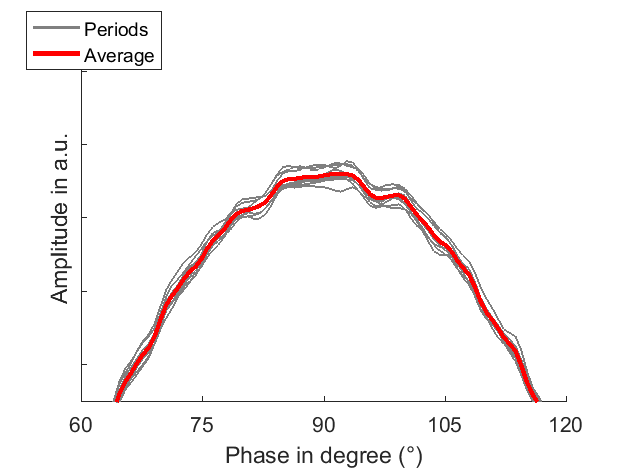
\includegraphics[width=\textwidth]{./img/distortion.png}
    \caption{Distortion}\label{fig:distortion}
    \end{subfigure}
    \begin{subfigure}{.5\textwidth}
    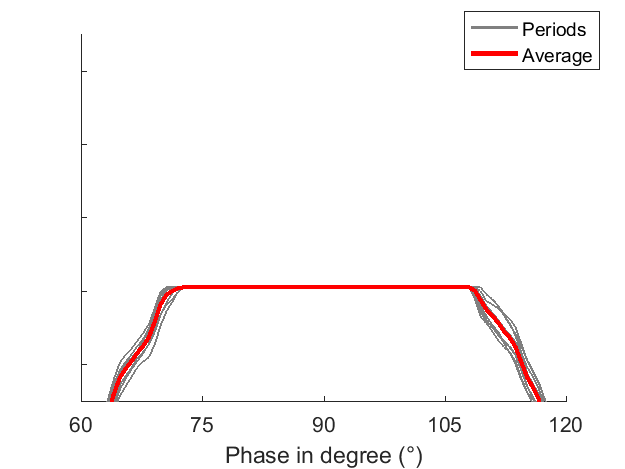
\includegraphics[width=\textwidth]{./img/saturation.png}
    \caption{Saturation}\label{fig:saturation}
    \end{subfigure}
    \caption{Examples for loss of sinusoidal fidelity}\label{fig:nonsinus}
\end{figure}

The temporally and spatially uneven impedance distribution has been suggested as cause of distortion, rendering the resulting waveform periodic, but non-sinusoidal. A major problem is amplifier saturation, i.e.\ the stimulation artifact exhibiting an amplitude to large for the dynamic range of the amplifier, causing the signal to be cut off and information to be lost.
Additionally, non-linearites in the amplifier slew rate can distort the shape even when the signal is close to the saturation threshold. Recently, non-linearities in how stimulators control the applied current has been suggest as further source of modulation~\citep{Neuling_2017}.

\subsection{Computational Demands}

Methods based on adaptive template construction and \gls{tpca}~\citep{Niazy_2005} have been explored for removal of  non-stationary and misshaped \gls{tacs} artifacts~\citep{Helfrich_2014}.  Consider that the process of template construction, the estimation of accurate weights for removal by template subtraction and the suqsequent removal of residual artifacts using \gls{tpca} is computationally cumbersome. Additionally, it often requires off-line analysis supported by visual inspection.
Such a multi-staged template-approach is therefore of limited utility for on-line artifact removal. Furthermore, critical evaluation has suggested that the residual artifact spans several principal components, and a sufficient artifact removal is therefore not possible with \gls{tpca} \citep{Noury_2016}.

\subsection{Rationale}

We were interested in development of a computationally fast approach, feasible for online artifact removal. At the same time, the approach was required to account for the dynamical modulation of the artifact amplitude, and the possibility of non-sinusoidal distortion and saturation. Ideally, the approach should allow to estimate physiological signals at the frequency of stimulation, even if physiological oscillations were phase-locked to the stimulation signal.

\section{Approach}

The main idea is that at any given time point $t$, the recorded signal $r(t)$ is a linear super\-position of a neurophysiological signal $n(t)$, the stimulation artifact $a(t)$ and a white noise term $e(t)$. The task is to recover $n(t)$ by estimating $a(t)$ and $e(t)$ and subtracting from $r(t)$.

\begin{eqnarray}
    r(t) = n(t) + a(t) + e(t)\\
    n(t) = r(t) - a(t) - e(t)
\end{eqnarray}

\subsection{Periodic Estimation}
Assume that the~\gls{tacs} artifact were \emph{non-sinusoidal}, but \emph{stationary and periodic}. At the same time, assume that neurophysiological signals $n$ were absent, but the noise term $e$ remains~\eqref{eq:Shapeless}. Then, we could estimate the amplitude of $a$ at any time-point $t$ by using the recorded signal $r$ from any~\gls{tacs} one period length $\tau_a$ earlier~\eqref{eq:ArtSim}.

\begin{align}
    r(t) & = a(t) + e(t)\label{eq:Shapeless}\\
    \hat{a}(t) & = r(t-\tau_a)\label{eq:ArtSim}
\end{align}

Consider that the white noise term $e$ is superpositioned on $r$, and  $\langle e\rangle$ converges asymptotically to zero with increased sample size.

\subsubsection{Averaging Comb Filter}
An optimal approach to achieve an unbiased estimate of the amplitude of a stationary artifact would therefore be to average across as many earlier periods as possible~\eqref{eq:Average}. Subsequently, this estimate can be used to  remove the artifact from $r$. Subtraction of a delayed version of the signal is also known as comb filter.

\begin{equation}
    \hat{a}(t) = \sum_{n=1}^{N} \frac{r(t - (n~\tau_a))}{N}\label{eq:Average}
\end{equation}

\subsubsection{Superposition of moving averages}
Please note also that averaging across neighbouring periods $M$~\eqref{eq:SMA} has been suggested before and termed~\gls{sma} by~\cite{Kohli_2015}.

\begin{equation}
    \hat{a}(t) = \sum_{n-M/2}^{n+M/2} \frac{r(t - (n~\tau_a))}{M+1}\label{eq:SMA}
\end{equation}

Consider that the approach using only past values~\eqref{eq:Average} returns a causal filter. A causal filter would be able to remove the artifact without the delay of $\frac{M \tau_a}{2}$ necessary for~\gls{sma}. Additionally, if applied offline on time-flipped signals, a causal filter has the potential to mininize distortion of neurophsyiological signals by mirroring a strong event-related potential.

\subsection{Temporal Weighting}

In real applications, stimulation duration is limited and computational contraints exist. This is reflected by the fact that we have to use a finite number for $N$. More importantly, the artifact amplitude has been described to be non-stationary  and dynamically modulated~\citep{Noury_2016}.
For such real applications, equation~\eqref{eq:Average} can return a biased estimate, depending on whether the integral of this modulation over the time-period $N\times\tau_a$ converges to zero.
One attempt to tackle with this issue can be the use of a time-dependent weighting function instead of a constant $N$~\eqref{eq:Weighted}, with the weighting function designed to reduce a possible bias.

\begin{equation}
    \hat{a}(t) = \sum_{n=1}^{N} w_n r(t - (n~\tau_a))\label{eq:Weighted}
\end{equation}

Note that if the dynamical modulation is known or can be estimated sufficiently, an optimal weighting function can be constructed. Sadly, we rarely know the time course of artifact modulation in advance. Furthermore, the dynamical system governing the modulation can be difficult or impossible to estimate. There are several options to approximate the dynamical system, and justify a generic weighting function.

\subsubsection{Linear Weighting}

One solution is linearization, e.g.\ using a linear decreasing weighting function. This can be implemented by using the triangular number $T_N = \frac{N(N+1)}{2}$ for a given $N$ as a normalizing constant. Hence, equation~\eqref{eq:Linear} returns weights for earlier periods based on their linear temporal delay.

\begin{equation}
    w_n = \frac{2(N+1-n)}{N(N+1)}\label{eq:Linear}
\end{equation}

\subsubsection{Exponential Weighting}

Motivated by the fact that exponentials are an essential building block of signal processing, an alternative approach could be an exponential weighting function. The time constant $\tau_e$ of an exponential controls its decay across time. To maintain the shape across different $N$, we consider it reasonable to normalize the time constant $\tau_e$ by $N$~\eqref{eq:NormTau}. Hence, equation~\eqref{eq:Expo} returns weights for earlier periods based on their exponential temporal delay.

\begin{equation}
    w_n = \frac{e^{x(N-n)}}{k}\label{eq:Expo}
\end{equation}
\begin{subequations}
with the following shape parameters
\begin{align}
    x   & = \frac{\tau_e}{N}\label{eq:NormTau}\\
    k   & = \sum_{n=1}^{N}e^{nx} = \frac{1-e^{Nx}}{1-e^{x}}-1
\end{align}
\end{subequations}

\subsection{Computational Implementation}

We implemented the approach in Matlab 2016b on a Windows 10 machine. First, we constructed a kernel based on the respective weighting functions~\eqref{eq:Weighted} and desired memory, or number of periods $N$. This kernel was then used to remove the artifact in a recording by convolution.
We wanted to evaluate the behavior of the filter in off-line analysis on simulated and real data and decided to use zero-padding for ease of computation.

\subsubsection{Exemplary Kernels}
Peruse the following exemplary kernels constructed for a sampling rate of 1KHz, a stimulation frequency of 10 Hz and a periodic memory of 5.  Please note that we intened to test the approach in offline analysis. To keep the kernel causal, we centered it by left-padding with zeros.

\begin{figure}[hbtp]
\begin{subfigure}{.33\textwidth}
    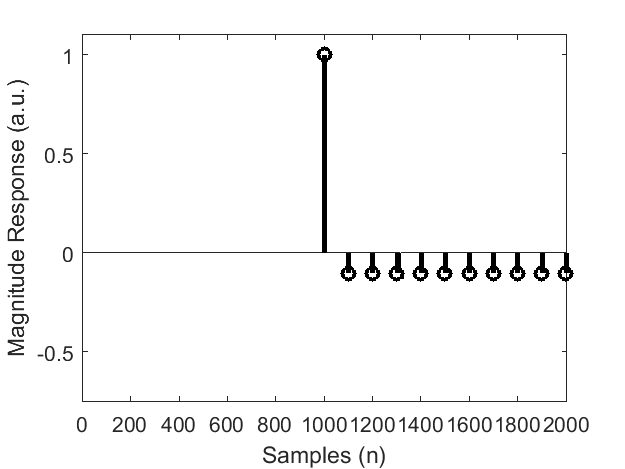
\includegraphics[width=\textwidth]{img/kernel_ave.png}\\
    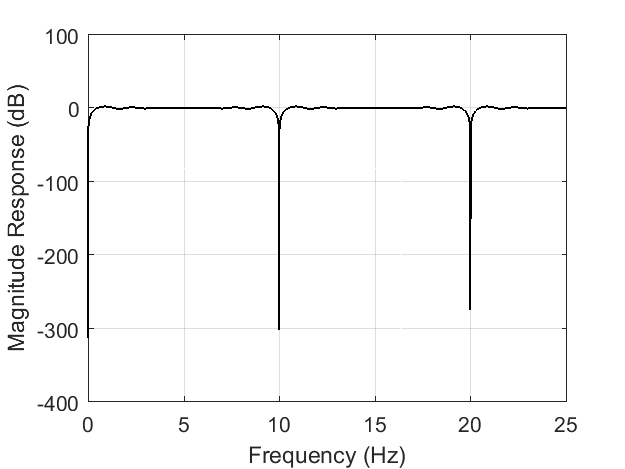
\includegraphics[width=\textwidth]{img/mag_ave.png}
    \caption{Average Combing Kernel}\label{fig:AverageKernel}
\end{subfigure}
\begin{subfigure}{.33\textwidth}
    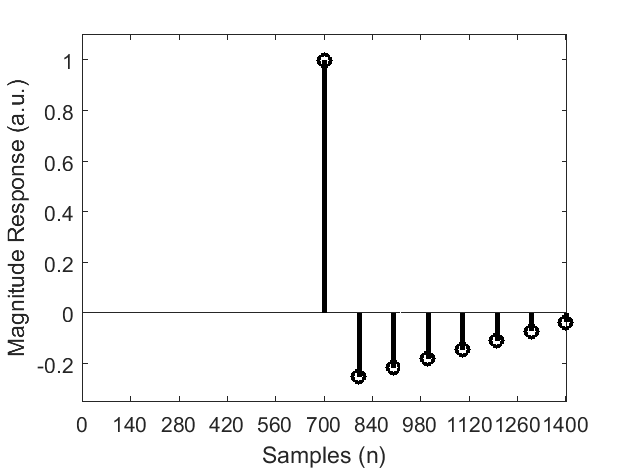
\includegraphics[width=\textwidth]{img/kernel_linear.png}\\
    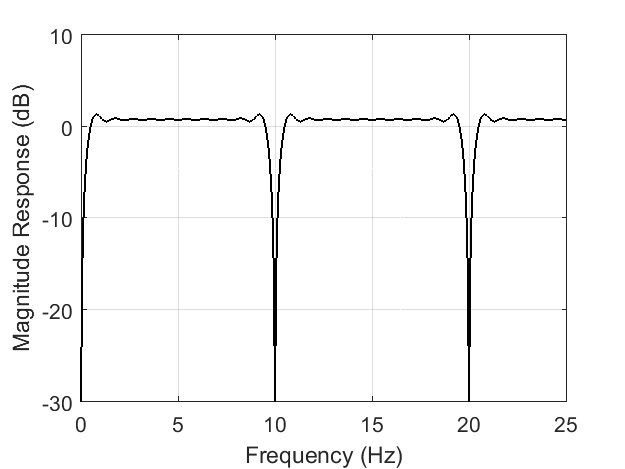
\includegraphics[width=\textwidth]{img/mag_linear.png}
    \caption{Linear Weighted Kernel}\label{fig:LinearKernel}
\end{subfigure}
\begin{subfigure}{.33\textwidth}
    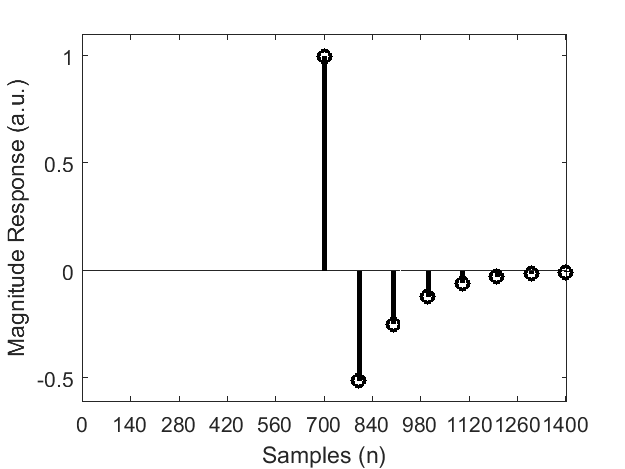
\includegraphics[width=\textwidth]{img/kernel_exp.png}\\
    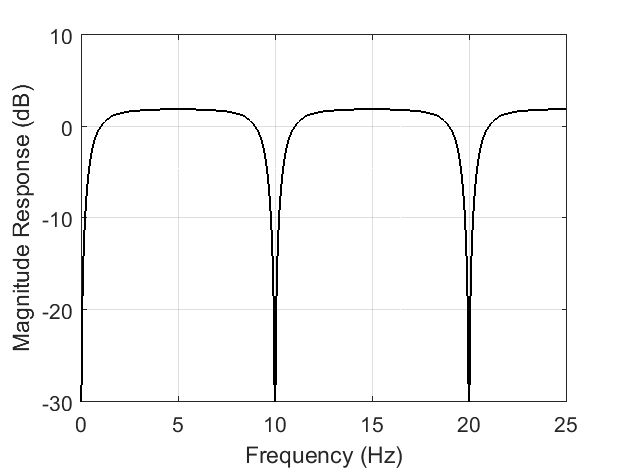
\includegraphics[width=\textwidth]{img/mag_exp.png}
    \caption{Exponential Weighted Kernel}\label{fig:ExponentialKernel}
\end{subfigure}
\caption{Exemplary Kernels and their respective Magnitude Response}\label{fig:ExemplaryKernels}
\end{figure}

As you can see from figure~\ref{fig:ExemplaryKernels}, the (numerically calculated) magnitude responses of the three approaches are almost identical.
The key characteristic of each kernel of them is the strong supression of signals at the target frequency defined by the period length and its integer multiples.
Yet, note the slightly higher ringing in the passband for the average combing kernel~\ref{fig:AverageKernel} compared to e.g.\ the smooth transition for the exponential weighted kernel~\ref{fig:ExponentialKernel}.

\subsubsection{Code Repository}











\section{Evaluation}

\section{Conclusion}


\bibliographystyle{apalike-oadoi}
\bibliography{sample}

\end{document}
